\documentclass{scrartcl}
\usepackage{localstyle}

\title{Authorization Logic For App Policies}
\subtitle{Second Year Report}
\author{Joseph Hallett}
\date{\today{}}

\begin{document}
\maketitle{}

\begin{abstract}
  Despite the proliferation of mobile apps and app markets there have been very few tools to help users find the apps which are appropriate to their own own privacy and security concerns.
  The large amount of personal data associated with phones makes them attractive targets for advertisers.
  Current methods for enforcing privacy and security policies require care by users to only pick the apps which meet their policies and to control and manually pick privacy settings.
  We propose that by using an authorization logic we can, to some degree, automate the decision making process.
  We describe the AppPAL policy language and show how it can be used as a framework for making decisions about apps on the basis of policy in a precise manner.
  The evaluation algorithm is discussed and we show how we have used AppPAL to see the extent users follow mobile privacy policies.
  We discuss potential avenues for future research and give a plan producing a PhD thesis.
\end{abstract}

\section{Motivation}

Mobile devices let users pick the apps they want to run.
App stores offer a wide range of software for users to choose.
Users pick particular apps for a variety of reasons:
  ordering in the store~\citep{Prata:2012in},
  reviews and privacy concerns~\citep{Kelley:2013kc},
  and security rules from their employer.

Finding the right apps can be tricky:
  users need to work out which apps are well written, which are not going to abuse their data, which ones will work in the way they want
  and to find the apps which suit how they want to use their device.
This can be difficult as it isn't obvious how apps use the data each has access to.

People fall into patterns when thinking about the privacy issues around apps~\citep{Sadeh:2014vq}.
By capturing these patterns explicitly as policies they can be enforced automatically.
This reduces the burden on users to decide which apps they want.
Security-savvy users may design policies themselves: these could be shared with others or used in organisation-wide curated app stores.

Companies have policies about how phones should be used by employees.
With \emph{bring your own device} schemes employees use their personal devices for work.
IT departments in these companies may need to create policies so that the devices can be used securely with company information.
Ensuring compliance is often left to the employees.
By using an authorization logic we believe these policies can be enforced automatically.
This reduces the burden on users to ensure compliance, and IT departments to check it.


\section{Aims and Constraints}

We are developing a policy language to express and enforce user policies for mobile apps and explore the policies users want and use.
We then aim to use this language as a framework for describing and comparing different policies; when previously they were only described using natural language.
Current approaches require users to make their decisions about which apps on a case-by-case basis.
When user's are asked to repeatedly make security decisions they can become fatigued and start to make poorer decisions.
Using an authorization logic we can help guide users to make the correct decision for them, and perhaps make some decisions for them.
This would reduce user fatigue and help users make more consistent decisions.

By writing user policies in a formal language we can compare them precisely.
This helps us explain the differences between different kinds of users and the security models in the operating system.

We have taken the SecPAL~\citep{Becker:2006vh} authorization logic and modified it create a new instantiation called \emph{AppPAL}.
AppPAL describes app installation policies for Android, and supports delegation and trust relationships as well as dynamic running of static analysis tools.

\subsection{The AppPAL Language}

AppPAL is an instantiation of SecPAL~\citep{Becker:2006vh} for describing app policies.
SecPAL is a logic of authorization for access control decisions in distributed systems.
It has a clear and readable syntax, as well as rich mechanisms for delegation and constraints.
SecPAL has already been used as a basis for other policy languages in areas such as privacy preferences~\citep{Becker:2009ula} and data-sharing~\citep{Aziz:2011vt}.
We believe SecPAL can also be applied to mobile devices~\citep{Hallett:2014un}.
We present AppPAL as a new version of SecPAL, targeting apps on mobile devices.

In \autoref{lst:corporate} we describe a compliance scenario where we have used AppPAL to model the security policy.
Alice works for Emma the employer.
As part of her job Alice uses her personal phone for work (a \ac{BYOD} scheme) which Emma allows with some conditions about what she may run for security.
These conditions are that:
\begin{itemize}
  \item Apps mustn't leak her location.
  \item Apps must come from a reputable source like the Google Play Store.
  \item Apps must be checked using the corporate anti-virus tool.
\end{itemize}

\begin{figure}
    \begin{lstlisting}[numbers=left,
                       escapeinside={@}{@}]
"alice" says "emma" can-say inf
  App isRunnable. @\label{lst:corporate_1}@

"emma" says App isRunnable @\label{lst:corporate_2}@
  if "no-tracking-policy" isMetBy(App),
     "reputable-policy" isMetBy(App),
     "anti-virus-policy" isMetBy(App).

"emma" says
  "reputable-policy" isMetBy(App) @\label{lst:corporate_3}@
      if App isReputable.

"emma" says "google-play" can-say 0
  App isReputable. @\label{lst:corporate_4}@

"emma" says "anti-virus-policy" isMetBy(App) @\label{lst:corporate_5}@
  if App isAnApp
  where
    mcAfeeVirusCheck(App) = false.

"emma" says "no-location-permissions"
  can-act-as "no-tracking-policy". @\label{lst:corporate_6}@

"emma" says
  "no-location-permissions" isMetBy(App) @\label{lst:corporate_7}@
    if App isAnApp
    where
      hasPermission(App, "LOCATION")=false.
\end{lstlisting}
\caption{Example AppPAL policy demonstrating various language features.}
\label{lst:corporate}
\end{figure}

To implement the rules Alice makes the following assertions.
In \autoref{lst:corporate_1} Alice gives Emma the ability to specify whether an \code{App} (a variable) \code{isRunnable} (a predicate).
She allows her to delegate the decision further if she chooses (\code{can-say inf}).
Next in \autoref{lst:corporate_2} Emma specifies her concerns as policies to be met (the \code{isMetBy()} predicate that takes an app as its argument).
If Emma can be convinced all these policies are met then he will say the \code{App isRunnable}.
In \autoref{lst:corporate_3} and \autoref{lst:corporate_4} Emma specifies that an app meets the \code{reputable-policy} if the \code{App isReputable};
  with \code{"google-play"} specified as the decider of what is buyable or not.
This time Google is not allowed to delegate the decision further (\code{can-say  0}).
In other words Google is not allowed to specify Amazon as a supplier of apps as well.
Google must say what is buyable directly for Emma to accept it.
Emma specifies the \code{"anti-virus-policy"} in \autoref{lst:corporate_5}.
Here we use a constraint.
When checking the policy the \code{mcAfeeVirusCheck} should be run on the \code{App}.
Only if this returns \code{false} will the policy be met.
To specify the \code{"no-tracking-policy"} Emma says that the \code{"no-location-permissions"} rules implement the \code{"no-tracking-policy"} (\autoref{lst:corporate_6}).
Emma specifies this in \autoref{lst:corporate_7} by checking the app is missing two permissions.

When Alice wants to install a new app (\code{com.facebook.katana}) on her phone.
To meet Emma's policy the AppPAL policy checker needs to collect statements to show the app meets the \code{isRunnable} predicate.
Specifically it needs:
\begin{itemize}
  \item\code{"emma" says "com.facebook.katana" isAnApp.}
    A simple typing statement that can be generated for all apps as they are encountered.
    This helps keep the number of  assertions in the policy low aiding readability.
  \item\code{"google-play" says "com.facebook.katana" isReputable.}
    Required to convince Emma the app came from a reputable source.
    It should be able to obtain this statement from the Play store as the app is available there.
  \item\code{"emma" says "anti-virus-policy" isMetBy("com.facebook.katana").}
    She can obtain this by running the \ac{av} program on her app.
  \item\code{"emma" says "no-locations-permissions" isMetBy("com.facebook.katana").}
    Needed to show the App meets Emma's no-tracking-policy.
    Emma will say this if after examining the app the location permissions are missing.
\end{itemize}
These last two statements require the checker to do some extra checks to satisfy the constraints.
To get the third statement it must run the \ac{av} program on her app and check the result.
The results from the \ac{av} program may change with time as it's signatures are updated;
  so the checker must re-run this check every time it wants to obtain the statement connected to the constraint.
For the forth statement the checker needs to check the permissions of the app.
It could accomplish this by looking in the \texttt{MANIFEST.xml} inside the app itself.

One scenario we could imagine is Alice wanting to check the apps when she wants to run them.
Alternatively we could imagine Emma wanting a personalised app store where all apps sold meet her policy.
With AppPAL this can be implemented by taking an existing store and selectively offering only the apps which will meet the user's policy.
This gives us a \emph{filtered store}.
From an existing set of apps we produce a personalised store that meets a pre-defined policy.

\subsection{AppPAL Evaluation}

\begin{figure}
\[
% AC, D ⊧ A says B can-act-as C   AC, D ⊧ A says C verbphrase
% ----------------------------------------------------------- (can-act-as)
%                 AC, D ⊧ A says B verbphrase
\infer[\text{\footnotesize\textsf{can-act-as}}]{
  AC, D \models \text{\tt A says B verbphrase}}{%
  AC, D \models \text{\tt A says B can-act-as C} & %
  AC, D \models \text{\tt A says C verbphrase}}
\]
\[
% AC, ∞ ⊧ A says B can-say D fact   AC, D ⊧ B says fact
% ----------------------------------------------------- (can-say)
%                   AC, ∞ ⊧ A says fact
\infer[\text{\footnotesize\textsf{can-say}}]{
  AC, \infty \models \text{\tt A says fact}}{%
  AC, \infty \models \text{\tt A say B can-say $D$ fact} & %
  AC, D \models \text{\tt B says fact}}
\]
\[
% (A says fact if fact₁, …, factₖ, c) ∈ AC
% AC, D ⊧ A says factᵢθ  ∀i ∈ {1…k}    ⊧cθ    vars(factθ) = ∅
% ----------------------------------------------------------- (cond)
%                    AC, D ⊧ A says factθ
\infer[\text{\footnotesize\textsf{cond}}]{
  AC, D \models \text{\tt A says fact$\theta$}}{
  \begin{array}{c}
    (\text{\tt A says fact if fact$_1$, \ldots, fact$_k$ where c}) \in AC \\
    \forall i \in 1\cdots k.\;AC, D \models \text{\tt A says fact$_i\theta$}
  \end{array} &
  \models \mathtt{c}\theta &
  \text{\sl vars}(\text{\tt fact$\theta$}) = \emptyset}
\]
\caption{SecPAL's evaluation rules.}
\label{fig:rules}
\end{figure}

To evaluate AppPAL we use an evaluation algorithm derived from the evaluation rules of SecPAL (\autoref{fig:rules}).
Unlike SecPAL we do not make use of a DatalogC based translation evaluation method as their aren't libraries implementing DatalogC for Android.
In \autoref{lst:eval} we show pseudocode for the evaluation of AppPAL assertions.
The full algorithm is implemented in Java and runs on Android as well as the desktop.

We believe it to be correct (that is to say the tests pass), but formally proving the algorithm is equivalent to the inference rules is future work.

\begin{figure}
  \begin{minipage}{0.5\linewidth}
    \begin{lstlisting}[language=Ruby,basicstyle=\footnotesize\ttfamily]
class Evaluation
  # Start a new evaluation session by loading an assertion context
  def init(ac)
    # Implicit functions are statements that can be derived without additional AppPAL predicates.  They are marked as derivable, as a statement formed from from one is derivable by inspection.
    Evaluation.implicit_functions.each {|f|
      this.derivable.add f
    }

    this.ac = ac
    this.ac.assertions.each {|a|
      # Premptively add an assertion to the results table if it is a ground fact
      rt.add a if a.is_ground? and a.constraint.isTrue?
      # Add predicate to the derivable table if it is not ground (i.e. there is a potential variable assignment which could be true)
      this.derivable.add a if (not a.is_ground?) and a.consequent.is_a_predicate?
    }
  end

  # Evaluate a query at an assertion depth
  def evaluate(q, d)
    # Fetch answer if we know it.
    rt.get q, d if rt.has q, d

    # Don't try and evaluate anything we cannot derive.
    return Failure if q.consequent.is_a_predicate and not this.derivable.contains q

    # Apply the cond rule, or the cansay or canactas rule, else fail.
    this.rt.mark_unfinished q, d
    this.cond q, d or
    this.cansay_canactas q, d or
    this.failure q, d
  end
  \end{lstlisting}
\end{minipage}
  \begin{minipage}{0.5\linewidth}
    \begin{lstlisting}[language=Ruby,basicstyle=\footnotesize\ttfamily]
  # The cond rule
  def cond(q, d)
    # Evaluate an implicit fact.
    return evaluate_implicit q if this.implicit q

    # Try and find a rule in the AC to prove the query
    this.ac.each  {|a|
      u = headUnify q, a
      if u.sucessful
        a_ = u.substitution a
        if a_.consequent.vars.size == 0
          result = check_antecedents_and_constraint q, d
          return Success if result.is_good
        end
      end
    }

    return Failure # We couldn't find a proof
  end

  # For the cansay and canactas rules we search for a valid delagator (cansay) or role (canactas) that can replace the subject of the query.  The AC is preprocessed to find potential speakers (constants who say something) and subjects (constants about which something is said) to avoid unnecessary searches.
  def cansay_canactas(q, d)
    this.ac.constants.each {|c|
      if this.ac.is_subject? c
        result = canactas q, d
        return result if result.is_good?
      else if this.ac.is_speaker? c
        result = canactas q, d
        return result if result.is_good?
      end
    }
    return Failure
  end
end
\end{lstlisting}
\end{minipage}
\caption{Pseudocode for AppPAL evaluation.}
\label{lst:eval}
\end{figure}

\subsection{User Behaviour}

Current versions of Android display lists of permissions of apps when the app is first installed.
These permissions control access to APIs for accessing personal information and hardware devices (such as the camera).
For users checking permissions is the only means of controlling what data apps have access to.
Currently the permissions, once granted, cannot be revoked by users without uninstalling the app.
In the next version of Android individual permissions will be able to be revoked at any time for any non-system app.

In a user study of 725 Android users, Lin~\etal{} found four patterns that characterise user privacy preferences for apps~\citep{Sadeh:2014vq}.
The \emph{Conservative} (C) users were uncomfortable allowing an app access to any personal data for any reason.
The \emph{Unconcerned} (U) users felt okay allowing access to most data for almost any reason.
The \emph{Advanced} (A) users were comfortable allowing apps access to location data but not if it was for advertising reasons.
Opinions in the largest cluster, \emph{Fencesitters} (F), varied but were broadly against collection of personal data for advertising purposes.
We wrote AppPAL policies to describe each of these behaviours as increasing sets of permissions:
% The policies are of increasing strictness, each banning more permissions.
These simplify the patterns discovered. %~\citep{Sadeh:2014vq}.
But AppPAL constraints can describe richer policies than permission sets.


\begin{table}
  \label{tab:lin}
\newcommand{\tabtitle}[1]{\textbf{\footnotesize #1}}
\begin{center}
  \begin{tabular}{ r l l l l }
%                                       & \rothead{Conservative} & \rothead{Advanced} & \rothead{Fencesitter} & \rothead{Unconcerned} \\
    \toprule
    \tabtitle{Policy}                  & \tabtitle{C}           & \tabtitle{A}       & \tabtitle{F}          & \tabtitle{U}          \\
    \midrule
    \lstinline{GET_ACCOUNTS}           & \xmark                 & \xmark             & \xmark                & \xmark                \\
    \lstinline{ACCESS_FINE_LOCATION}   & \xmark                 & \xmark             & \xmark                &                       \\
    \lstinline{READ_CONTACT}           & \xmark                 & \xmark             & \xmark                &                       \\
    \lstinline{READ_PHONE_STATE}       & \xmark                 & \xmark             &                       &                       \\
    \lstinline{SEND_SMS}               & \xmark                 & \xmark             &                       &                       \\
    \lstinline{ACCESS_COARSE_LOCATION} & \xmark                 &                    &                       &                       \\
    \bottomrule
  \end{tabular}
\end{center}
\caption{Simplification of privacy profiles identified by Lin~\etal{}}
\end{table}

Installation data was taken from a partially anonymized\footnote{Users are replaced with incrementing numbers, app names are replaced with hashes to protect sensitive names.} database of installed apps captured by Carat~\citep{Oliner:2013ht}.
By calculating the hash of known package names we see who installed what.
The initial database has over 90,000 apps and 55,000 users.
On average each user installed around 90 apps each; 4,300 apps have known names.
Disregarding system apps (such as \texttt{com.android.vending}) and very common apps (Facebook, Dropbox, Whatsapp, and Twitter) we reduced the set to an average of 20 known apps per user.
To see some variations in app type, we considered only the 44,000 users who had more than 20 known apps.
% We removed users for whom we knew less than 20 ; for whom we didn't have a representative sample of installations.
Using this data, and the apps themselves taken from the Google Play Store and Android Observatory~\citep{Barrera:2012iba}, we checked which apps satisfied which policies.


\begin{figure}\centering
  \begin{subfigure}[b]{0.45\linewidth}\centering
    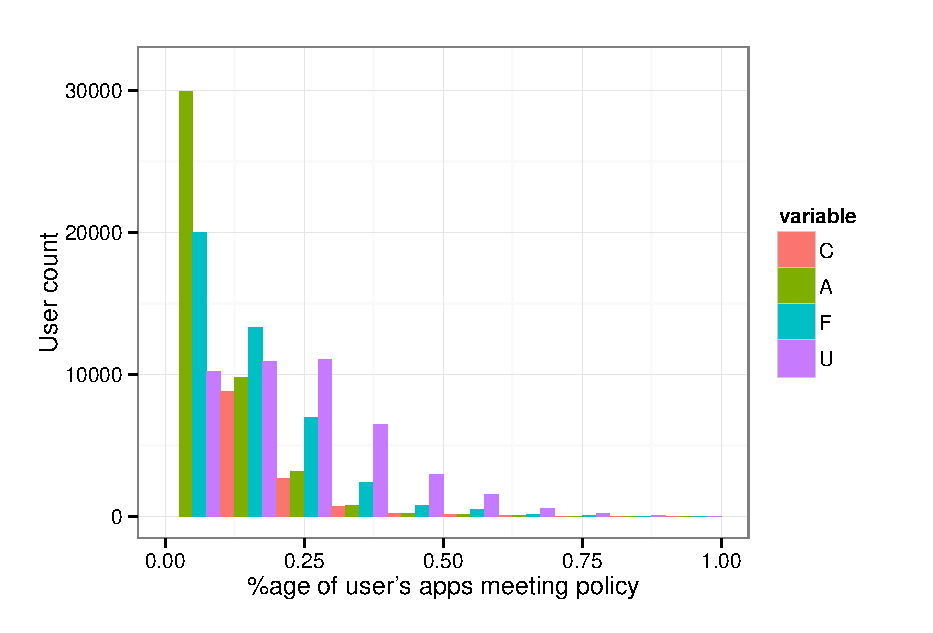
\includegraphics[width=\linewidth]{./images/lin-poster.eps}
    \caption{Use of policies modelling user behaviour.}
    \label{fig:lin}
  \end{subfigure}
  \begin{subfigure}[b]{0.45\linewidth}\centering
    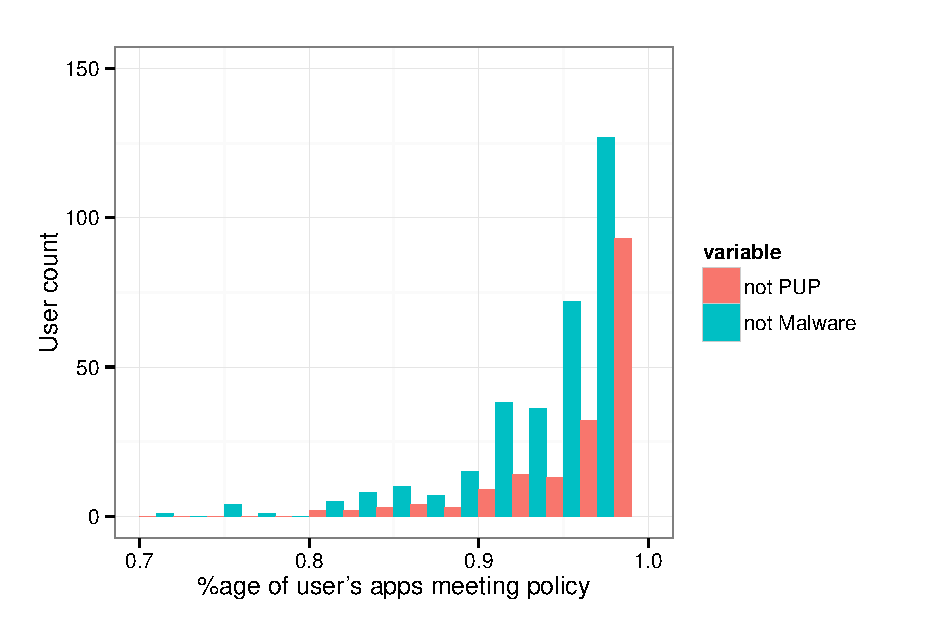
\includegraphics[width=\linewidth]{./images/malware-poster.eps}
    \caption{Installation rates of malware.}
    \label{fig:malware}
  \end{subfigure}
  \begin{subfigure}[b]{0.45\linewidth}\centering
    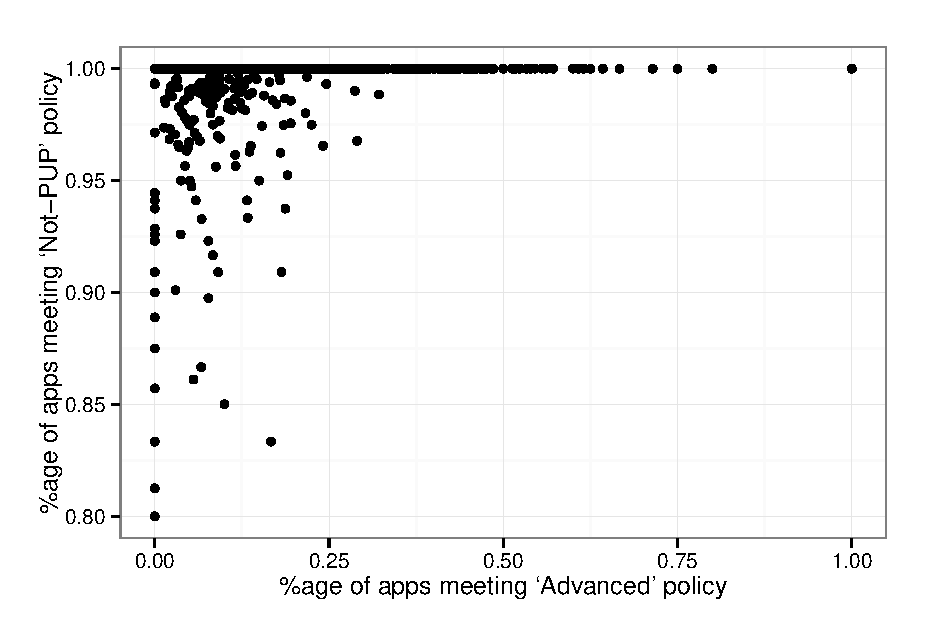
\includegraphics[width=\linewidth]{./images/advanced-vs-malware.eps}
    \caption{Comparison of users following the advanced policy to those not installing PUPs.}
    \label{fig:advancedvspup}
  \end{subfigure}
  \caption{Graphs showing user uptake of policies.}
\end{figure}

Figure~\ref{fig:lin} shows that the very few users follow these policies, but a few users who do seem to be installing apps meeting these policies most of the time.
For the unconcerned policy (the most permissive) only 1,606 users (4\%) had 50\% compliance;
and only 120 users (0.3\%) had 80\% compliance.
For the stricter conservative policy only 60 users were complying half the time, and just 7 more than 80\% of the time.
This suggests that while users may have privacy preferences the majority are not attempting to enforce them.

We found 1\% of the users had a PUP or malicious app installed.
Figure~\ref{fig:malware} shows that infection rates for PUPs and malware is small.
A user is 3 times more likely to have a PUP installed than malware.
Only 9 users had both a PUP and malware installed.
Users who were complying more than half the time with the conservative or advanced policies complied with the malware or PUP policies fully.
This is significant (P-value $< 0.05$) and suggests that users who pick their apps carefully are less likely to experience malware.


\subsection{Means of Enforcement}

Since AppPAL is implemented as a library we have tried to develop prototype applications that allow us to use AppPAL as a tool to explore policies.
These are not finished tools, but provide a start point for finding the appropriate places to use AppPAL and play with policies.

The \emph{AppPAL Checker} (\autoref{fig:apppal-checker}) is an Android app that checks installed apps against user privacy policies~\citep{Sadeh:2014vq}.
The checking is done on device, and shows the user which apps meet the policy and which do not.
Checking is limited to set policies, though this could be extended to support arbitrary policies.

The AppPAL checker could be used as part of a user study to gain information about user's installs as well as provide a framework for testing different UIs and AppPAL policies.
It is also useful for checking the performance of the AppPAL evaluator on various devices.

The \emph{AppPAL Store Generator} (\autoref{fig:genstore}) allows a policy designer to generate a store where the apps sold meet an arbitrary policy.
The generator produces a webapp that provides a simple store selling apps and with categories defined by the policy.
This gives us a framework for filtering apps on the basis of policies and presenting them to users.
This could be used as part of a user study where we ask users to search for apps on the basis of policies.
It could be used to compare time and success rate at searching for apps meeting a policy with AppPAL and with existing methods.
Currently it is limited to generating stores with a fixed policy but this can be changed as needs be.

\begin{figure}\centering
  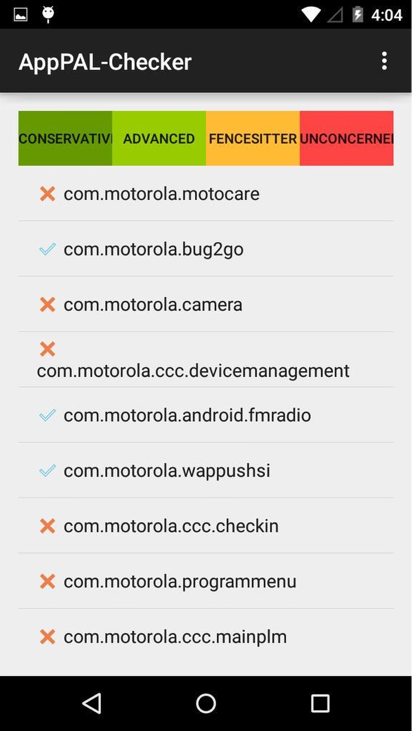
\includegraphics[width=0.3\linewidth]{./images/apppal-checker.png}
  \caption{The AppPAL checker showing the Apps installed on a device and whether they meet a conservative privacy policy.}
  \label{fig:apppal-checker}
\end{figure}
\begin{figure}\centering
  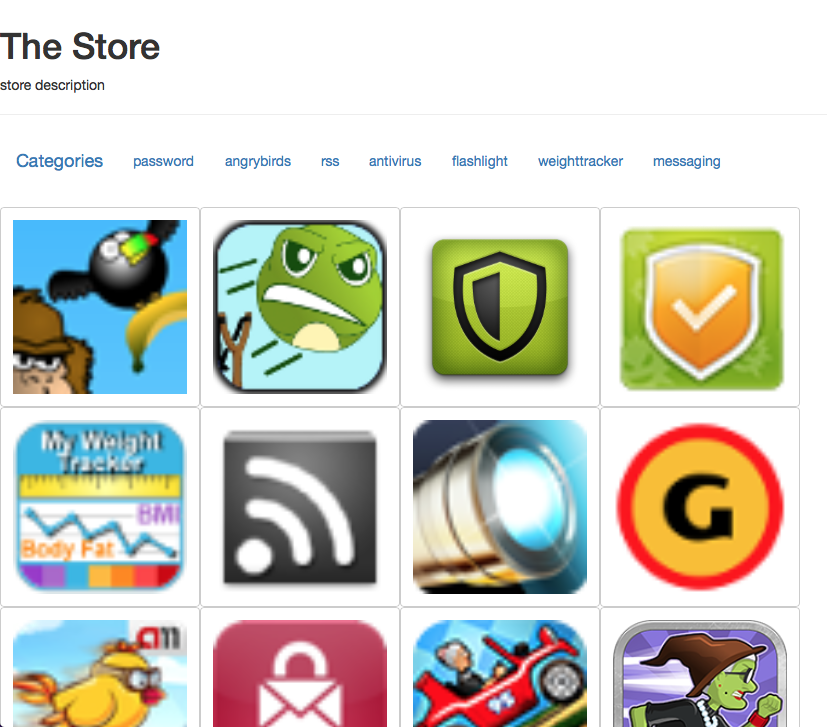
\includegraphics[width=0.7\linewidth]{./images/genstore.png}
  \caption{Example store generated by the AppPAL store generator.}
  \label{fig:genstore}
\end{figure}

\section{Thesis Outline}

\begin{quote}
\emph{\emph{Hypothesis.}  Automatic tools and policy languages would provide a
better means of enforcement for mobile device policies than existing mechanisms
which rely on manual inspection.}
\end{quote}

\begin{enumerate}
  \item Introduction
  \item Mobile Ecosystems
    \begin{description}
      \item[App stores and mobile app deployment]
        \hfill
        \begin{itemize}
          \item Introduce app stores and current development practices.
          \item Show the differences between different market places and the platforms (iOS vs Android).
        \end{itemize}
      \item[Android Security Model]
        \hfill
        \begin{itemize}
          \item Introduce the android permissions model and how different apps can access functionality provided by the platform.
          \item Show how app signing works.
        \end{itemize}
      \item[Android policies]
        \hfill
        \begin{itemize}
          \item Introduce the need for policies and the motivation for the PhD.
          \item Show how users do not seem to be following their privacy policies.
          \item Explain how some companies have mobile device policies, and how users are frustrated with data leaks.
          \item Show existing tools, such as Kirin, and explain why they're not good enough.
        \end{itemize}
    \end{description}
  \item AppPAL
    \begin{description}
      \item[The need for a policy language]
        \hfill
        \begin{itemize}
          \item Introduce scenarios where AppPAL can be used to enforce a policy
          \item Show trust relationships between different principals (a user at work).
          \item Start to introduce the language.
        \end{itemize}
      \item[Design and implementation of AppPAL]
        \hfill
        \begin{itemize}
          \item Formally present the language, as an instantiation of SecPAL.
          \item Show evaluation algorithm.
          \item Maybe show correctness proofs?
          \item Maybe compare performance on different devices?
        \end{itemize}
      \item[Deployment]
        \hfill
        \begin{itemize}
          \item Show applications using AppPAL.
          \item Stores generated by policy.
          \item On device policy checking.
          \item Device configuration by policy (if we can get access to Android M features)
        \end{itemize}
    \end{description}
  \item Evaluation
    \begin{description}
      \item[Learning policies from user data]
        \hfill
        \begin{itemize}
          \item Use Carat/other data to learn current user policies.
          \item Express them using AppPAL.
          \item Compare to user privacy preferences.
          \item Are they being enforced?
        \end{itemize}
      \item[User study]
        \hfill
        \begin{itemize}
          \item Can users use AppPAL to find apps that meet a policy faster and more accurately than through search alone?
          \item Do users prefer using a policy tool to find apps meeting their policies?
        \end{itemize}
      \item[Case study]
        \hfill
        \begin{itemize}
          \item Show how we can take a corporate policy and enforce it using AppPAL.
          \item Show the language is expressive enough to describe real policy scenarios.
          \item Show it works in \emph{the real world}.
        \end{itemize}
    \end{description}
  \item Related Work
  \item Future Work
\end{enumerate}

\section{Evaluation}

To evaluate the AppPAL system we need to show that existing mechanisms for policy enforcement are failing to give users the power to readily enforce their policies;
  that users can make use of and like the system;
  that AppPAL can actualy solve policy enforcement problems in the real world.

\subsection{Learning policies from user data}

The privacy paradox is that whilst people tend to have opinions about privacy and security, they rarely seem to implement their preferences.
Even security experts tend not to follow all their own advice~\citep{Ion:2015uq}.
\citeauthor{Sadeh:2014vq} identified various privacy preferences different users had.
When we looked at app installation data, however, we found that the most users didn't seem to follow them~\citep{Hallett:2015ty}.

By using app installation data we should be able to learn what policies users are applying in practice.
These can be described using AppPAL and used to make a precise comparison between the policies users use, and those they want.
We believe there will be significant differences between the two policies.
This will be used as evidence that existing policy mechanisms are not good enough, as well as help design new policies for users.

\subsection{User study on usability of AppPAL}

A user study should evaluate whether AppPAL is a better solution to policy checking than existing methods.
The study should look at whether user's can find apps matching a given policy both quicker and more accurately than with existing tools.
It should also look at whether user's can understand policies and the implications of finding or not finding a policy is met.
Finally it should also look at whether users like the system, and whether they would use it.

This research would answer whether AppPAL is a good solution.
If we find that it is faster and more accurate than existing solutions this suggests that authorization logics offers an improvement over existing methods when it comes to picking apps.
If users like it, then this suggests that it is a good solution and the language offers good features for the problems users have.
If we find that it is not a good fit, and that users do not like it then this should motivate changes to the language, or it should be further hidden from users under an additional layer.
A negative reaction may indicate that authorization logics are not a good solution here, and further research should look at why when they have fit so many other areas.

The SOUPS conference may make an ideal target for the publication of any papers drawn from this work.
SOUPS publishes several papers based on user studies each year and has shown a strong interest in moblile privacy policies.
We have had some success there in 2015 with a poster.

\subsection{Case study on applying AppPAL to a compliance scenario}

Having an authorization logic model and enforce a real world policy shows the limitations and expressivity of a language.
It also shows that it is applicable to current compliance problems and solves \emph{real world problems} rather than just the policies we have learnt from user behaviour.

A natural source of these real world policies is corporate \ac{BYOD} policies, where employers describe restrictions on the useage of mobile devices in the workplace.
The \ac{NIST} have published recomendations for mobile device security and \ac{BYOD} in the workplace~\citep{Souppaya:2013jf,Scarfone:2009vy}.
Translating the mobile device relevant sections into AppPAL and showing their enforcement might make a good case study.
The study would focus on any difficulties in translating the policies and how much of the policy could be enforced automatically.

\bibliographystyle{plainnat}
\bibliography{report}
\end{document}
